\section{Initial Experiments}
Here I shall document the inital experiments I have performed with both GPT, and
Google Gemini \citet{gemini2023}. 

\subsection{Haskell Examples in Chat GPT}
I began by working on with Chat-GPT (GPT-4o), using small examples, a later
experiment will determine how to perform the same experiments using \kw{fluid}.
I gave example programs, asked it to demonstrate similar ones, culminating in it
generating an accessor function for a list of records. A presentation of the chat
log is shown in \figref{chatgpt-experiment}. 

\begin{figure}
   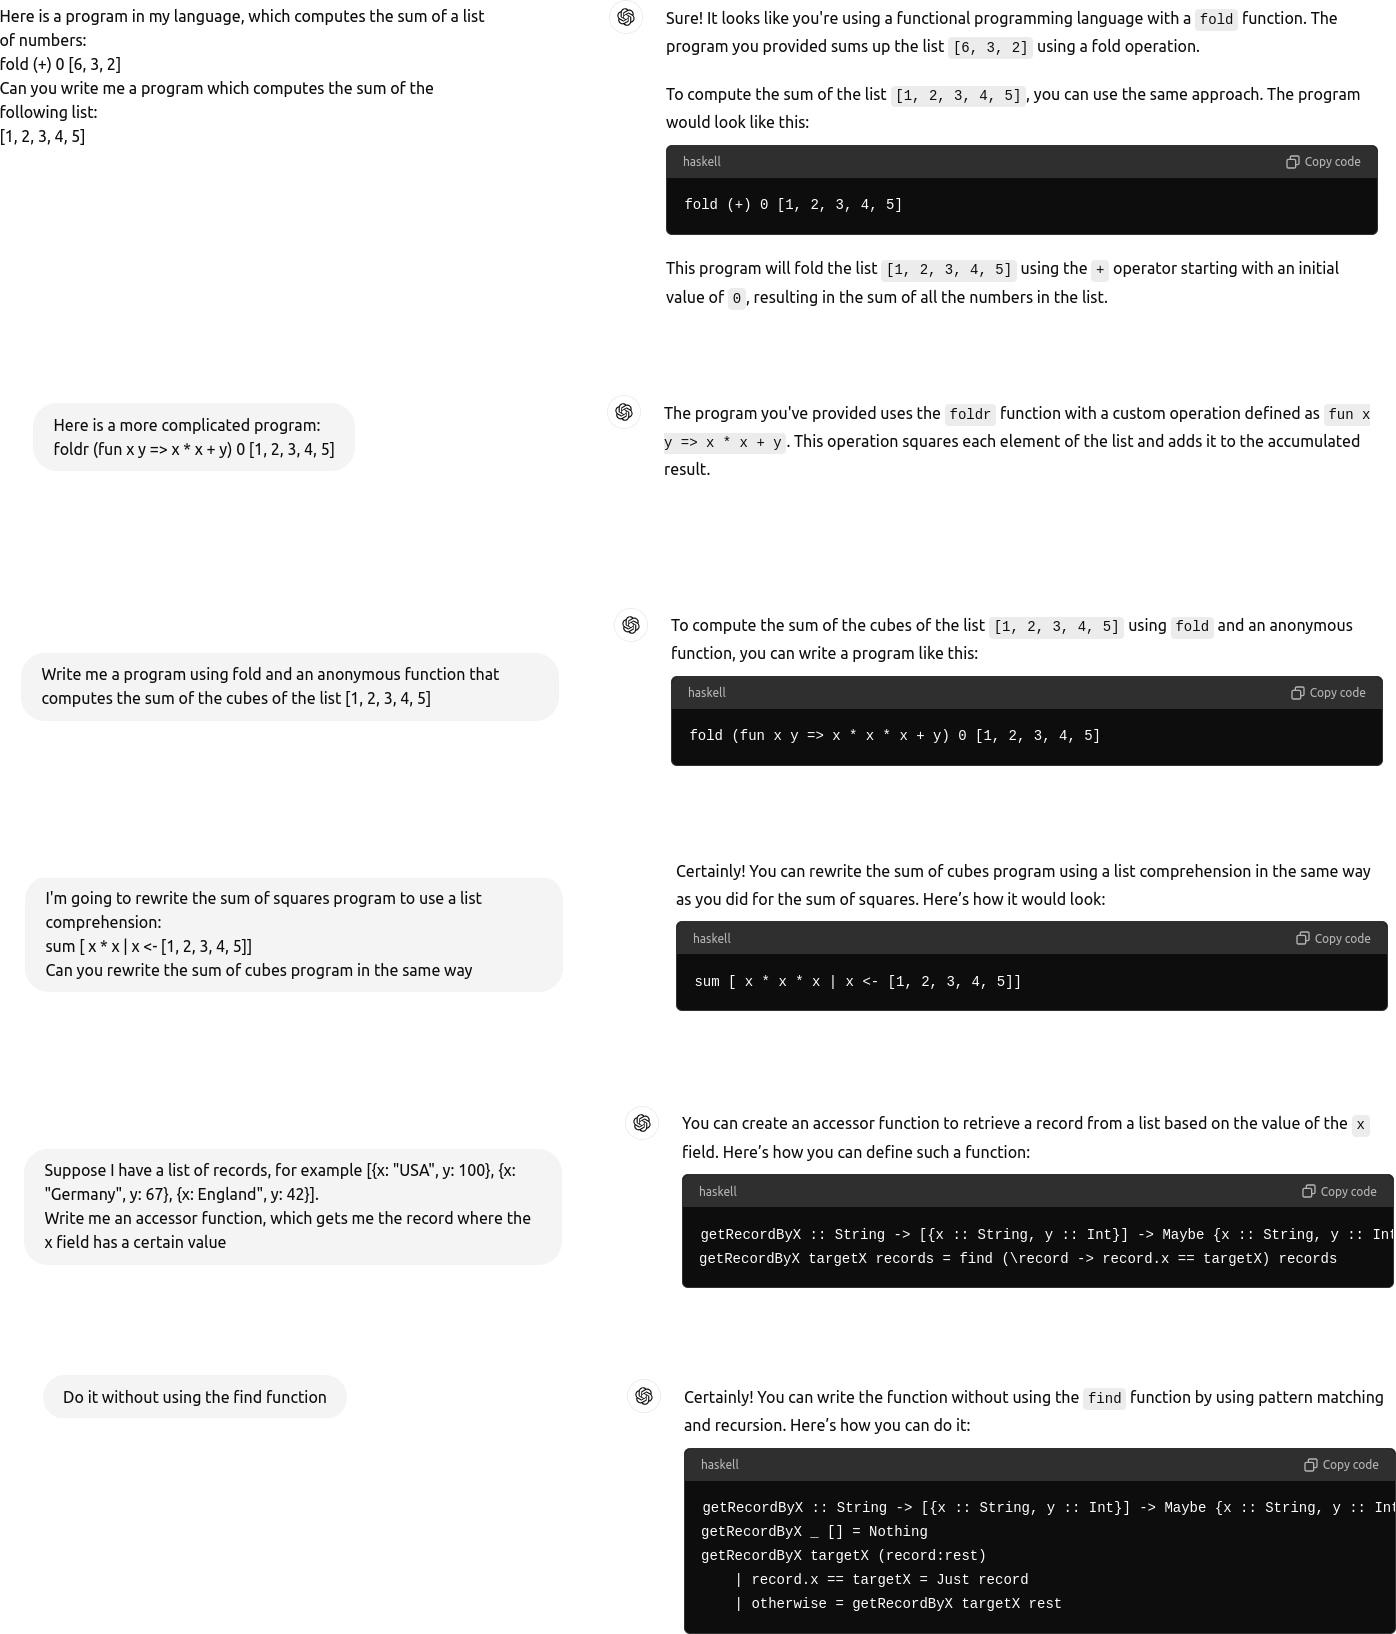
\includegraphics{fig/chat-gpt-experiment.png}
   \caption{Initial Chat-GPT experiment}
   \label{fig:chatgpt-experiment}
\end{figure}

\paragraph*{Initial notes: } without specifying the choice of language, 
Chat-GPT inferred that I was using a functional language, and stuck to 
a reasonable facsimile of Haskell for the duration of this experiment. 
It defaulted to a sensible Haskell style, including the use of type-annotations.
If we use Few-shot learning, or some other method to condition the model, I think
an initial challenge is going to be forcing it to write valid fluid code. 